\documentclass{beamer}

\usepackage[T1]{fontenc}
\usepackage[utf8]{inputenc}

\usepackage{lmodern}

\usepackage{mathtools,amssymb}

\usepackage{graphicx}
\usepackage{xcolor}
\usepackage{tikz}

\usepackage{booktabs}

\usepackage{appendixnumberbeamer}

\definecolor{red_UCM}{HTML}{b01131}
\usetheme{Berlin}
\useoutertheme{infolines}
\useinnertheme{rectangles}
\usecolortheme[named=red_UCM]{structure}
\setbeamercolor{alerted text}{fg=red_UCM}

\usetikzlibrary{calc, positioning}
\AtBeginSection[]{\begin{frame}\tableofcontents[currentsection]\end{frame}}
\setbeameroption{show notes}
\setbeamertemplate{note page}{\insertnote}
\addtobeamertemplate{note page}{}{\thispdfpagelabel{notes:\insertframenumber}}
\setbeamertemplate{navigation symbols}{}
\usebackgroundtemplate{\tikz[overlay,remember picture]\node[opacity=0.03125]at (current page.center){\includegraphics[scale=0.5]{images/UCM-logo.png}};}
\renewcommand\appendixname{Appendix}

\title[XXII GISC Workshop]{Evolving Safely: Adaptation and Phenotypic Diversity under Environmental and Demographic Constraints}
\author[]
{
  \texorpdfstring{{\large Mendívil Carboni, Marco\inst{1}}\\\vspace{1ex} Dinis Vizcaíno, Luis Ignacio\inst{1} (dir.) \and Mazo Torres, Juan José\inst{1} (dir.)}{Marco Mendívil Carboni}
} 
\institute[Universidad Complutense de Madrid]
{
  \inst{1}
  Grupo Interdisciplinar de Sistemas Complejos (GISC) and Departamento de Estructura de la Materia, Física Térmica y Electrónica, Universidad Complutense de Madrid
}

\begin{document}

\frame{\titlepage}

\begin{frame}
  \tableofcontents
\end{frame}

\section{Introduction and objectives}

\begin{frame}
  \begin{columns}
    \hfill
    \begin{column}{0.6\textwidth}
      \begin{block}{Motivation}
        \begin{itemize}
          \item \alert{Adaptation} in fluctuating \alert{environments} is not fully understood yet.
          \item Especially under \alert{population limitations}.
          \item Paradigmatic example of \alert{fluctuations in biological processes}.
        \end{itemize}
      \end{block}

    \end{column}
    \begin{column}{0.4\textwidth}
      \begin{figure}
        \frame{\includegraphics[scale=0.12]{images/changing-environment.jpg}}
      \end{figure}
    \end{column}
  \end{columns}

  \begin{block}{Objectives}
    \begin{itemize}
      \item Develop a minimal mathematical \alert{model} to study this problem.
      \item Model the emergence of \alert{bet-hedging} strategies in fluctuating environments.
      \item Quantify how the \alert{evolutionary outcome} depends on these constraints.
      \item Identify the main mechanisms shaping these results and seek ways to \alert{approximate} them.
    \end{itemize}
  \end{block}

  \note[item]{Adaptation in fluctuating environments is a \alert{central problem} in \alert{evolutionary biology}.}
  \note[item]{Natural populations experience fluctuating rather than constant environments.}
  \note[item]{We will use a minimal mathematical model, \alert{not a detailed biological one}.}
  \note[item]{To investigate this, we will use \alert{numerical simulations}.}
  \note[item]{The main objective is to understand \alert{how populations adapt in fluctuating environments under demographic constraints}.}
  \note[item]{A key question is whether these outcomes can be described using an \alert{effective notion of fitness}.}
\end{frame}

\section{The model: a Markov process}

\begin{frame}
  \begin{block}{System state}
    \begin{itemize}
      \item \alert{Environment}: $e\in\{1,2\}$
      \item \alert{Population}: $N$ agents, each one characterized by:
            \begin{itemize}
              \item \alert{phenotype}: $\phi\in\{A,B\}$
              \item \alert{strategy}: $s(\phi)$ (probability distribution)
            \end{itemize}
    \end{itemize}
  \end{block}

  \note[item]{\alert{Continuous-time} Markov process describing a population evolving in a fluctuating environment, that we will solve numerically using the \alert{Gillespie algorithm}.}
  \note[item]{The population starts with an initial number of agents \alert{$N_{\text{ini}}$}.}
  \note[item]{The environment is a \alert{discrete variable} that changes according to some transition rates.}
  \note[item]{The phenotype takes \alert{discrete values} as well.}
\end{frame}

\begin{frame}
  \begin{block}{Dynamics}
    \begin{itemize}
      \item \alert{Environment}: transition rates \alert{$\omega_t(e,e')$}
      \item \alert{Population}: environment- and phenotype-dependent birth and death rates \alert{$\omega_b(e,\phi)$} and \alert{$\omega_d(e,\phi)$}
      \item \alert{Evolution}: offsprings inherit the parent's strategy, mutations occur with probability \alert{$p_{\text{mut}}$}
      \item \alert{Constraint}: population size \alert{capped at $N_{\text{ini}}$}
    \end{itemize}
  \end{block}
  \vfill
  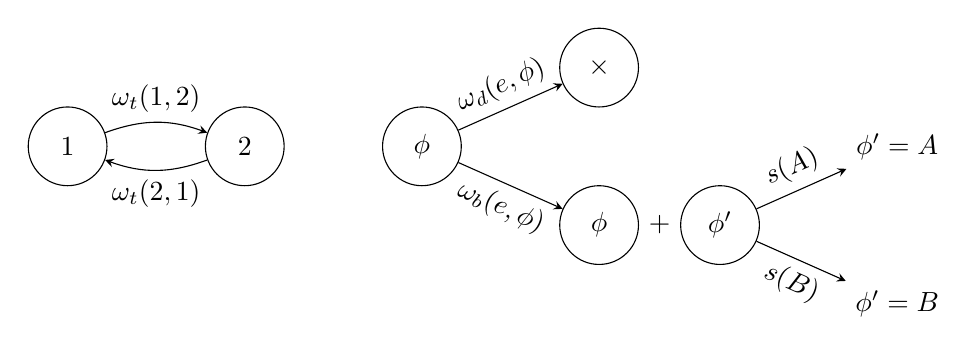
\begin{tikzpicture}[>=stealth, node distance=2.25cm]
    \node (e1) [draw, circle, minimum size=1cm]{$1$};
    \node (e2) [draw, circle, minimum size=1cm, right of=e1] {$2$};
    \draw[->, bend left=20]
    (e1) to node[above] {$\omega_t(1,2)$} (e2);
    \draw[->, bend left=20]
    (e2) to node[below] {$\omega_t(2,1)$} (e1);
    \node[draw, circle, minimum size=1cm, right of=e2] (agent) {$\phi$};
    \node[right of=agent, yshift=+1cm, draw, circle, minimum size=1cm] (death) {$\times$};
    \node[right of=agent, yshift=-1cm, draw, circle, minimum size=1cm] (parent) {$\phi$};
    \node[right=0cm of parent] (plus) {$+$};
    \node[right=0cm of plus, draw, circle, minimum size=1cm] (offspring) {$\phi'$};
    \node[right of=offspring, yshift=+1cm] (A) {$\phi'=A$};
    \node[right of=offspring, yshift=-1cm] (B) {$\phi'=B$};
    \draw[->]
    (agent) -- node[sloped, midway, above] {$\omega_d(e,\phi)$} (death);
    \draw[->]
    (agent) -- node[sloped, midway, below] {$\omega_b(e,\phi)$} (parent);
    \draw[->]
    (offspring) -- node[sloped, midway, above] {$s(A)$} (A);
    \draw[->]
    (offspring) -- node[sloped, midway, below] {$s(B)$} (B);
  \end{tikzpicture}

  \note[item]{When an agent reproduces, the \alert{offspring's phenotype is drawn from the parent's strategy}.}
  \note[item]{\alert{Offspring inherit} the same \alert{phenotypic strategy} as their parent, allowing natural selection to act on strategies.}
  \note[item]{To allow \alert{evolution}, mutations are introduced: with a small probability at duplication, an agent's strategy \alert{mutates to a new random strategy}.}
  \note[item]{The total population size is \alert{capped at its initial value}, introducing a demographic constraint.}
\end{frame}

\begin{frame}
  \begin{block}{Parameters -- resistant vs. persistent}
    \begin{table}
      \begin{tabular}{c c c}
        \toprule
        symbol             & name                         & value                                                        \\
        \midrule
        $\omega_t(e,e')$   & environment transition rates & $\begin{psmallmatrix}-1.0&+1.0\\+1.0&-1.0\end{psmallmatrix}$ \\
        \addlinespace
        $\omega_b(e,\phi)$ & birth rates                  & $\begin{psmallmatrix}1.0&0.2\\0.0&0.0\end{psmallmatrix}$     \\
        \addlinespace
        $\omega_d(e,\phi)$ & death rates                  & $\begin{psmallmatrix}0.0&0.0\\1.0&0.1\end{psmallmatrix}$     \\
        \addlinespace
        $p_{\text{mut}}$   & mutation probability         & $0.001$                                                      \\
        \addlinespace
        $N_{\text{ini}}$   & initial number of agents     & $100$                                                        \\
        \bottomrule
      \end{tabular}
    \end{table}
  \end{block}

  \begin{block}{Types of simulations}
    \begin{enumerate}
      \item \alert{\texttt{fixed}}: \alert{common} initial strategy $s(\phi)_{\text{ini}}$, \alert{not evolving} ($p_{\text{mut}}=0$).
      \item \alert{\texttt{evol}}: \alert{common} initial strategy $s(\phi)_{\text{ini}}$, \alert{evolving}.
      \item \alert{\texttt{evol(r)}}: \alert{independent random} initial strategies, \alert{evolving}.
    \end{enumerate}
  \end{block}

  \note[item]{We restrict ourselves to the case of \alert{two} environments and two phenotypes.}
  \note[item]{Environmental transition rates are equal and set to one, making \alert{both environments equally likely} for simplicity.}
  \note[item]{The environment alternates between a \alert{good} and a \alert{bad} state.}
  \note[item]{The \alert{resistant} phenotype grows fast in the good environment but dies quickly in the bad one, while the \alert{persistent} phenotype grows slowly but survives much better in bad conditions.}
  \note[item]{In \alert{fixed} simulations, all agents share the same strategy and \alert{evolution is suppressed}.}
  \note[item]{In \alert{evol} simulations, agents initially share a strategy, which evolves through \alert{mutation and selection}.}
  \note[item]{In \alert{evol(r)} simulations, agents start with independent random strategies, which then evolve.}
  \note[item]{Comparing the results of these three cases reveals the properties of the \alert{strategies} favored by selection, as we will see next.}
\end{frame}

\section{Results: phenotypic diversity and safe strategies}

\begin{frame}
  \begin{columns}
    \hfill
    \begin{column}{0.45\textwidth}
      \begin{block}{Observables}
        \begin{itemize}
          \item Average growth rate $\langle\mu\rangle$
          \item Total extinction rate $r_{\text{ext}}$
        \end{itemize}
      \end{block}
      \begin{block}{Take-home message}
        \alert{Growth-maximization} $\neq$ \alert{extinction-minimization}
      \end{block}
    \end{column}
    \begin{column}{0.55\textwidth}
      \begin{figure}
        \frame{\includegraphics[scale=0.75]{../sims/asymmetric/plots/strat_phe_0_i/avg_growth_rate.pdf}}
      \end{figure}
      \begin{figure}
        \frame{\includegraphics[scale=0.75]{../sims/asymmetric/plots/strat_phe_0_i/extinct_rate.pdf}}
      \end{figure}
    \end{column}
  \end{columns}

  \note[item]{The population growth rate is defined as \alert{$\Delta N/(N\Delta t)$}.}
  \note[item]{The number of extinctions is recorded to compute the total extinction rate.}
  \note[item]{These figures show the dependence of growth and extinction rates on the \alert{initial strategy} for different simulation types.}
  \note[item]{For \alert{evol(r)} simulations there is no common initial strategy, so they appear as strategy-independent horizontal lines.}
  \note[item]{Focusing on \alert{fixed} simulations we see that growth maximization and extinction minimization clearly \alert{do not coincide}.}
  \note[item]{Maximum growth occurs for strategies dominated (about \alert{80\%}) by the \alert{resistant} phenotype, while extinction is minimized by fully \alert{persistent} strategies.}
  \note[item]{Both \alert{evol} and \alert{evol(r)} simulations converge to similar growth and extinction rates, largely \alert{independent of the initial strategy}.}
  \note[item]{This indicates convergence toward a common \alert{evolutionary attractor}.}
\end{frame}

\begin{frame}
  \begin{columns}
    \hfill
    \begin{column}{0.45\textwidth}
      \begin{block}{Observables}
        \begin{itemize}
          \item Average strategy $\langle s(A)\rangle$
          \item Distribution of strategies $p(s(A))$
        \end{itemize}
      \end{block}
      \begin{block}{Evolutionary outcome}
        \begin{itemize}
          \item Convergence to a \alert{common average strategy}.
          \item \alert{Independent} of initial conditions.
        \end{itemize}
      \end{block}
      \begin{block}{Take-home message}
        Evolution selects a \alert{compromise} between growth-maximization and extinction-minimization.
      \end{block}
    \end{column}
    \begin{column}{0.55\textwidth}
      \begin{figure}
        \frame{\includegraphics[scale=0.75]{../sims/asymmetric/plots/strat_phe_0_i/avg_strat_phe_0.pdf}}
      \end{figure}
      \begin{figure}
        \frame{\includegraphics[scale=0.75]{../sims/asymmetric/plots/strat_phe_0_i/dist_strat_phe_0.pdf}}
      \end{figure}
    \end{column}
  \end{columns}

  \note[item]{We also compute the \alert{instantaneous standard deviation} of the strategy across agents.}
  \note[item]{Because strategies and the phenotype distribution are \alert{two-dimensional and normalized}, only one component is independent.}
  \note[item]{Both \alert{evol} and \alert{evol(r)} simulations converge to preety much the \alert{same average strategy}.}
  \note[item]{This indicates the presence of a \alert{stable attractor} in the space of strategies.}
  \note[item]{The \alert{strategy is common to almost all agents} at each instant, and thus talking about a \alert{common strategy} is meaningful.}
  \note[item]{This justifies comparing evolutive simulations with fixed-strategy simulations.}
  \note[item]{The \alert{histogram} of strategies however shows a bigger dispersion over time and across runs, but with a clear \alert{well-defined mean}.}
  \note[item]{The \alert{time-series} analysis will clarify the different kinds of dispersion.}
  \note[item]{The secondary peak directly reflects the \alert{initial strategy}, while the main peak is initial-condition independent.}
  \note[item]{The \alert{selected strategy} lies \alert{between} the growth-maximizing and extinction-minimizing strategies.}
\end{frame}

\begin{frame}
  \begin{columns}
    \hfill
    \begin{column}{0.45\textwidth}
      \begin{block}{Observables}
        \begin{itemize}
          \item Distribution of phenotypes $p(A)$
          \item Distribution of the number of agents $p(N/N_{\text{ini}})$
        \end{itemize}
      \end{block}
      \begin{block}{Actual phenotype distribution}
        \begin{itemize}
          \item \alert{Distribution of phenotypes} $\neq$ \alert{strategy}.
        \end{itemize}
      \end{block}
      \begin{block}{Population-size fluctuations}
        \begin{itemize}
          \item Population is \alert{usually} close to the \alert{maximum size $N_{\text{ini}}$}.
        \end{itemize}
      \end{block}
    \end{column}
    \begin{column}{0.55\textwidth}
      \begin{figure}
        \frame{\includegraphics[scale=0.75]{../sims/asymmetric/plots/strat_phe_0_i/dist_phe_0.pdf}}
      \end{figure}
      \begin{figure}
        \frame{\includegraphics[scale=0.75]{../sims/asymmetric/plots/strat_phe_0_i/dist_n_agents.pdf}}
      \end{figure}
    \end{column}
  \end{columns}

  \note[item]{I would also like to show some \alert{complementary results} that help clarify how the system behaves.}
  \note[item]{For a \alert{fixed strategy} and a \alert{fixed environment}, the phenotype distribution is easily obtained \alert{analytically} from the dominant eigenvector of a certain matrix.}
  \note[item]{The \alert{dash-dotted lines} show these two fixed-environment equilibria.}
  \note[item]{\alert{As expected}, with a \alert{fluctuating environment}, the observed phenotype distribution lies \alert{between} the two lines.}
  \note[item]{The \alert{main peak} corresponds to growth in the \alert{good environment}.}
  \note[item]{The \alert{secondary peak} reflects extended periods spent in the \alert{bad environment}.}
  \note[item]{Riskier strategies increase the weight of this secondary peak.}
  \note[item]{Since extinction corresponds to \alert{rare, large fluctuations} away from typical states near $N_{\text{ini}}$, a \alert{large-deviation} framework is a natural theoretical approach.}
\end{frame}

\begin{frame}
  \begin{columns}
    \hfill
    \begin{column}{0.45\textwidth}
      \begin{block}{Time series}
        \begin{itemize}
          \item \alert{Independent simulations} concatenated in time.
          \item Each run ends at an \alert{extinction event}.
          \item New runs start from a \alert{random initial condition}.
        \end{itemize}
      \end{block}
      \begin{block}{Strategy dynamics}
        \begin{itemize}
          \item Long \alert{plateaus} with a \alert{common strategy}.
          \item \alert{Abrupt switches} between strategies.
        \end{itemize}
      \end{block}
    \end{column}
    \begin{column}{0.55\textwidth}
      \begin{figure}
        \frame{\includegraphics[scale=0.75]{../sims/asymmetric/plots/time_series/n_extinct.pdf}}
      \end{figure}
      \begin{figure}
        \frame{\includegraphics[scale=0.75]{../sims/asymmetric/plots/time_series/avg_strat_phe_0.pdf}}
      \end{figure}
    \end{column}
  \end{columns}

  \note[item]{The \alert{vertical dotted lines} mark extinction times.}
  \note[item]{The lower panel shows the \alert{average strategy} as a function of time.}
  \note[item]{Error bands indicate the \alert{instantaneous dispersion} across agents and are barely visible.}
  \note[item]{As we anticipated, at any given time, the population shares a \alert{common strategy}, with negligible instantaneous dispersion.}
  \note[item]{This time-series also reveals a \alert{less obvious feature}: strategies remain almost \alert{constant over long times} and \alert{change abruptly} when a different strategy takes over.}
  \note[item]{Over long times and across runs, the explored strategies show a \alert{moderate dispersion}, consistent with the histogram we showed previously.}
\end{frame}

\begin{frame}
  \begin{columns}
    \hfill
    \begin{column}{0.45\textwidth}
      \begin{block}{Large population limit}
        With \alert{$N_{\text{ini}}=1000$}:
        \begin{itemize}
          \item Extinction is \alert{negligible}.
          \item Evolution converges to the \alert{growth-maximizing strategy}.
          \item Multiple similar \alert{strategies can coexist}.
        \end{itemize}
      \end{block}
      \begin{block}{Take-home message}
        \begin{itemize}
          \item The \alert{evolutionary outcome} depends on population size.
          \item \alert{Extinction risk} controls which strategies are selected.
        \end{itemize}
      \end{block}
    \end{column}
    \begin{column}{0.55\textwidth}
      \begin{figure}
        \frame{\includegraphics[scale=0.75]{../sims/extended/plots/strat_phe_0_i/avg_strat_phe_0.pdf}}
      \end{figure}
      \begin{figure}
        \frame{\includegraphics[scale=0.75]{../sims/extended/plots/strat_phe_0_i/dist_strat_phe_0.pdf}}
      \end{figure}
    \end{column}
  \end{columns}

  \note[item]{Increasing $N_{\text{ini}}$ strongly reduces the \alert{extinction risk} but does \alert{not} change the \alert{average growth rate}.}
  \note[item]{In this regime, the evolved strategy coincides with the \alert{growth-maximizing} one.}
  \note[item]{The evolutionary outcome therefore depends on population size through its effect on extinction.}
  \note[item]{Notice as well that the \alert{instantaneous dispersion} of strategies is still small, but larger than at small $N_{\text{ini}}$.}
  \note[item]{This reflects the coexistence of several \alert{similar strategies} within the population.}
  \note[item]{In contrast, the \alert{long-term dispersion} is reduced and comparable to the instantaneous one.}
\end{frame}

\section{Conclusions and future work}

\begin{frame}
  \begin{block}{Conclusions}
    \begin{itemize}
      \item Bet-hedging emerges \alert{naturally} from this minimal stochastic model.
      \item Our model yields populations with \alert{common or very similar strategies}.
      \item Evolution does \alert{not always maximize growth}.
      \item Demographic constraints shift selection toward \alert{safer strategies}.
    \end{itemize}
  \end{block}

  \begin{columns}
    \hfill
    \begin{column}{0.45\textwidth}
      \begin{block}{Future work}
        \begin{itemize}
          \item Measure the \alert{scaling} of extinction rates with $N_{\text{ini}}$.
          \item Derive an \alert{effective fitness} function combining growth and extinction.
          \item Extend the model to environment-dependent strategies (\alert{sensing}).
        \end{itemize}
      \end{block}
    \end{column}
    \begin{column}{0.55\textwidth}
      \begin{figure}
        \frame{\includegraphics[scale=0.75]{../sims/asymmetric/plots/strat_phe_0_i/fitness.pdf}}
      \end{figure}
    \end{column}
  \end{columns}

  \note[item]{At any given time the population is \alert{concentrated around a common strategy}, possibly with a small spread for large $N$.}
  \note[item]{The results suggest the existence of an \alert{effective fitness} incorporating extinction risk.}
  \note[item]{The figure shows a \alert{candidate objective function} combining average growth and extinction rate.}
  \note[item]{For the simulations presented here, its maximum coincides with the \alert{selected strategy}.}
  \note[item]{Deriving the \alert{effective fitness from theory} remains a key open problem.}
  \note[item]{\alert{Large deviations theory} appears as a natural framework to describe extinction events and their impact on selection.}
\end{frame}

\section*{Acknowledgments}

\begin{frame}
  \vfill
  \begin{center}
    \vfill
    \Large{Thank you for your attention.}
    \vfill
  \end{center}
  \vfill
  \begin{figure}
    \includegraphics[width=0.4\textwidth]{images/MICIU-logo.pdf}
  \end{figure}
\end{frame}

\appendix

\section*{Numerical methods}

\begin{frame}
  \begin{block}{Gillespie algorithm}
    \begin{equation*}
      \Omega(\mathbf{X})=\sum_{j=1}^M\omega_j(\mathbf{X})
    \end{equation*}
    \begin{equation*}
      \tau=\frac{1}{\Omega(\mathbf{X})}\ln\frac{1}{r_1},\ r_1\sim U(0,1)
    \end{equation*}
    \begin{equation*}
      \sum_{j=1}^{\mu-1}\omega_j(\mathbf{X})<r_2\Omega(\mathbf{X})\le\sum_{j=1}^{\mu}\omega_j(\mathbf{X}),\ r_2\sim U(0,1)
    \end{equation*}
    \begin{equation*}
      \mathbf{X}(t+\tau)=\mathbf{X}(t)+\boldsymbol{\nu}_\mu
    \end{equation*}
  \end{block}
\end{frame}

\section*{Symmetric parameters}

\begin{frame}
  \begin{columns}
    \hfill
    \begin{column}{0.5\textwidth}
      \begin{figure}
        \frame{\includegraphics[scale=0.75]{../sims/symmetric/plots/strat_phe_0_i/avg_growth_rate.pdf}}
      \end{figure}
      \begin{figure}
        \frame{\includegraphics[scale=0.75]{../sims/symmetric/plots/strat_phe_0_i/extinct_rate.pdf}}
      \end{figure}
    \end{column}
    \begin{column}{0.5\textwidth}
      \begin{figure}
        \frame{\includegraphics[scale=0.75]{../sims/symmetric/plots/strat_phe_0_i/avg_strat_phe_0.pdf}}
      \end{figure}
      \begin{figure}
        \frame{\includegraphics[scale=0.75]{../sims/symmetric/plots/strat_phe_0_i/dist_strat_phe_0.pdf}}
      \end{figure}
    \end{column}
  \end{columns}
\end{frame}

\begin{frame}
  \begin{columns}
    \hfill
    \begin{column}{0.5\textwidth}
      \begin{figure}
        \frame{\includegraphics[scale=0.75]{../sims/symmetric/plots/strat_phe_0_i/dist_phe_0.pdf}}
      \end{figure}
      \begin{figure}
        \frame{\includegraphics[scale=0.75]{../sims/symmetric/plots/strat_phe_0_i/dist_n_agents.pdf}}
      \end{figure}
    \end{column}
    \begin{column}{0.5\textwidth}
      \begin{figure}
        \frame{\includegraphics[scale=0.75]{../sims/symmetric/plots/time_series/n_extinct.pdf}}
      \end{figure}
      \begin{figure}
        \frame{\includegraphics[scale=0.75]{../sims/symmetric/plots/time_series/avg_strat_phe_0.pdf}}
      \end{figure}
    \end{column}
  \end{columns}
\end{frame}

\section*{Population-size dependence}

\begin{frame}
  \begin{columns}
    \hfill
    \begin{column}{0.5\textwidth}
      \begin{figure}
        \frame{\includegraphics[scale=0.75]{../sims/asymmetric/plots/n_agents_i/avg_strat_phe_0.pdf}}
      \end{figure}
      \begin{figure}
        \frame{\includegraphics[scale=0.75]{../sims/asymmetric/plots/n_agents_i/dist_strat_phe_0.pdf}}
      \end{figure}
    \end{column}
    \begin{column}{0.5\textwidth}
      \begin{figure}
        \frame{\includegraphics[scale=0.75]{../sims/symmetric/plots/n_agents_i/avg_strat_phe_0.pdf}}
      \end{figure}
      \begin{figure}
        \frame{\includegraphics[scale=0.75]{../sims/symmetric/plots/n_agents_i/dist_strat_phe_0.pdf}}
      \end{figure}
    \end{column}
  \end{columns}
\end{frame}

\section*{Mutation probability dependence}

\begin{frame}
  \begin{columns}
    \hfill
    \begin{column}{0.5\textwidth}
      \begin{figure}
        \frame{\includegraphics[scale=0.75]{../sims/asymmetric/plots/prob_mut/avg_strat_phe_0.pdf}}
      \end{figure}
      \begin{figure}
        \frame{\includegraphics[scale=0.75]{../sims/asymmetric/plots/prob_mut/dist_strat_phe_0.pdf}}
      \end{figure}
    \end{column}
    \begin{column}{0.5\textwidth}
      \begin{figure}
        \frame{\includegraphics[scale=0.75]{../sims/symmetric/plots/prob_mut/avg_strat_phe_0.pdf}}
      \end{figure}
      \begin{figure}
        \frame{\includegraphics[scale=0.75]{../sims/symmetric/plots/prob_mut/dist_strat_phe_0.pdf}}
      \end{figure}
    \end{column}
  \end{columns}
\end{frame}

\end{document}
